\documentclass[crop,class=article]{standalone}
%----------------------------Preamble-------------------------------%
\usepackage{pgfplots, tikz}             % Drawing/graphing tools.
\pgfplotsset{compat=1.9}                % Version of pgfplots.
%--------------------------Main Document----------------------------%
\begin{document}
    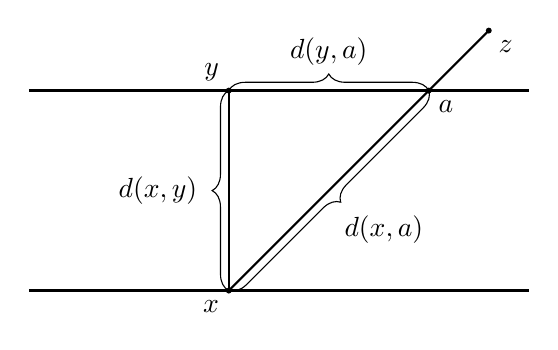
\begin{tikzpicture}
        \coordinate (x) at (0, 0);
        \coordinate (y) at (0, 1in);
        \coordinate (a) at (1in, 1in);
        \coordinate (z) at (1.3in, 1.3in);
        \draw[thick] (-1in, 0) to (1.5in, 0);
        \draw[thick] (-1in, 1in) to (1.5in, 1in);
        \draw[thick] (x) to (y);
        \draw[thick] (x) to (z);
        \draw[decorate, decoration={brace,amplitude=6pt}]
            (x) to node [xshift=-0.9cm] {$d(x,y)$} (y);
        \draw[decorate, decoration={brace,amplitude=6pt}]
            (a) to node [xshift=0.7cm,yshift=-0.5cm] {$d(x,a)$} (x);
        \draw[decorate, decoration={brace,amplitude=6pt}]
            (y) to node [yshift=0.5cm] {$d(y,a)$} (a);
        \draw[fill=black] (x) circle (0.3mm);
        \draw[fill=black] (y) circle (0.3mm);
        \draw[fill=black] (z) circle (0.3mm);
        \draw[fill=black] (a) circle (0.3mm);
        \node at (x) [below left] {$x$};
        \node at (y) [above left] {$y$};
        \node at (a) [below right] {$a$};
        \node at (z) [below right] {$z$};
    \end{tikzpicture}
\end{document}